\documentclass{article}
\usepackage{pgfplots}
\pgfplotsset{compat=1.17}

\begin{document}

The hyperbolic paraboloid $z = x^2 - y^2$ has a saddle point at the origin.

\begin{center}
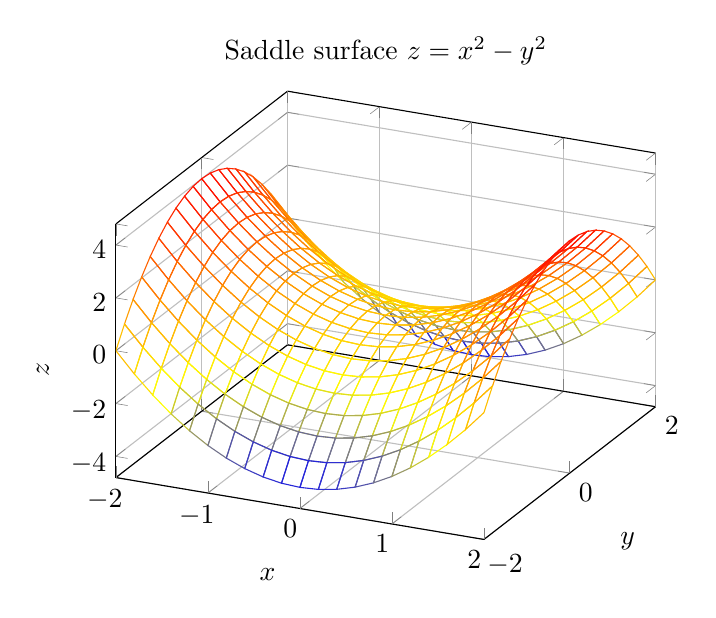
\begin{tikzpicture}
  \begin{axis}[
    title={Saddle surface $z = x^2 - y^2$},
    xlabel=$x$, ylabel=$y$, zlabel=$z$,
    grid=major,
  ]
    \addplot3[mesh, samples=21, domain=-2:2] {x^2 - y^2};
  \end{axis}
\end{tikzpicture}
\end{center}

\end{document}
